%% DTK Domain Model

\documentclass[letterpaper,12pt]{article}
\usepackage[top=1.0in,bottom=1.0in,left=1.25in,right=1.25in]{geometry}
\usepackage{appendix}
\usepackage{verbatim}
\usepackage{amssymb}
\usepackage{graphicx}
\usepackage{longtable}
\usepackage{amsfonts}
\usepackage{amsmath}
\usepackage{algpseudocode} 
\usepackage[usenames]{color}
\usepackage[
  naturalnames = true, 
  colorlinks = true, 
  linkcolor = black,
  anchorcolor = black,
  citecolor = black,
  menucolor = black,
  urlcolor = blue
]{hyperref}
\usepackage{listings}
\usepackage{textcomp}

%%---------------------------------------------------------------------------%%
\author{
  Stuart R. Slattery\\
  Department of Engineering Physics\\
  University of Wisconsin - Madison\\
  1500 Engineering Dr.\\
  Madison, WI 53716 \\
  \href{mailto:sslattery@wisc.edu}{\texttt{sslattery@wisc.edu}}
}

\date{\today}
\title{A Rendezvous-Based Domain Model for Data Transfer}
\begin{document}
\maketitle

%%---------------------------------------------------------------------------%%
\begin{abstract}
  In many physics applications, the concept of mesh is used to
  subdivide physical domain into a discrete representation to
  facilitate the solution of the model problems that describe
  it. Additionally, the concept of the field is used to apply degrees
  of freedom to the mesh as an additional means of
  discretization. With the increased development efforts in
  multiphysics simulation, adaptive simulations, and other multiple
  mesh problems, transferring fields and other data between meshes is
  a common operation. This document describes a domain model for mesh,
  fields, and data transfer based on the rendezvous algorithm and its
  implementation within the Data Transfer Kit software package.
\end{abstract}
\cleardoublepage
%%---------------------------------------------------------------------------%%
\tableofcontents
\clearpage
\listoffigures
\clearpage
\listoftables
\clearpage
\newpage

%%---------------------------------------------------------------------------%%
\section{Introduction}\label{sec:intro}
In many physics applications, it is often desired to transfer fields
(i.e. degrees of freedom or other data) between meshes that may or may
not conform in physical space. In addition, for massively parallel
simulations, it is typical that meshes not only do not conform
spatially, but also that their parallel decompositions do not
correlate and are independent of one another due to physics-based
partitioning requirements. As an example, this situation can occur in
multiphysics simulations where physics fields provide feedback between
solution iterations or adaptive mesh simulations where fields must be
moved between meshes after refining and coarsening. It is therefore
desirable to have a set of tools to relate two meshes of arbitrary
parallel decomposition such that fields and other data can be
transferred between them.

The Data Transfer Kit (DTK) is a software component designed to
provide parallel services for mesh repartitioning, mesh searching, and
data transfer based on the concept of the rendezvous decomposition
\cite{Plimpton_2004}. To achieve a component design for use with
arbitrary physics codes, general concepts of mesh and fields are
employed to provide access to these services. This document will
outline the concepts of mesh, fields, data transfer, and the
rendezvous decomposition and how they are modeled within the design of
DTK.

\clearpage

%%---------------------------------------------------------------------------%%
\section{Mesh}\label{sec:mesh}
In order to access DTK services, a subset of the information regarding
the mesh is required. This subset consists of nodes and their
coordinates, and elements and the nodes that construct them. In
addition, for meshes that contain multiple element topologies, the
concept of mesh blocked by element topology is utilized. For meshes
decomposed in parallel, the term global will be used to refer to
concepts that apply across the entire parallel domain while the term
local will be used to refer to concepts that only exist in the domain
of a single parallel process. A parallel communicator in the context
of DTK can be taken as a direct reference to a Message Passing
Interface (MPI) communicator.

\subsection{Mesh Nodes}\label{subsec:nodes}
Nodes are the lowest level geometric component of the mesh. All nodes
have a globally unique ordinal serving as an identification number for
the node in global operations. A node can have 1, 2, or 3 dimensions
but all nodes in a mesh must have the same dimension. To specify its
geometric position, each node has Cartesian (x,y,z) coordinates. A
node must provide only the coordinates for the specified node
dimension, no more or no less (e.g. a 2 dimensional node must provide
x and y coordinates but not a z coordinate). A node may be repeated
any number of times across the parallel domain with unlimited local
and global instances. However, every node with the same globally
unique ordinal must have the same coordinates. As an example, consider
figure~\ref{fig:mesh_nodes} depicting a series of nodes contained in
the mesh. Each node is provide a globally unique ordinal and set of 3
dimensional coordinates.

\begin{figure}[htpb!]
  \centering
  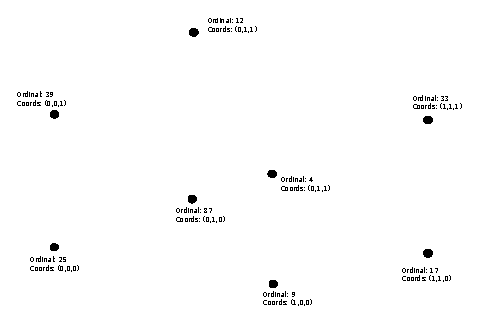
\includegraphics[width=5in]{hex_nodes.eps}
  \caption{\sl Basic node description for a mesh. Each node is
    required to have a unique global ordinal, a specified
    dimensionality, and Cartesian coordinates cooresponding to that
    dimensonality. The nodes in this example are 3 dimensional.}
  \label{fig:mesh_nodes}
\end{figure}

\subsection{Mesh Elements}\label{subsec:elements}
Elements are the second level of abstraction in the mesh above
nodes. All elements have a globally unique ordinal serving as an
identification number for the element in global operations. This
globally unique ordinal can be the same as a globally unique ordinal
for a node in the mesh as DTK distinguishes between nodes and
elements. An element has a topology defining its physical structure
(e.g. tetrahedron, hexahedron, etc.) and a number of nodes needed to
generate that topology. Elements are constructed from nodes via a
connectivity list. The connectivity list for a particular element will
contain the unique node global ordinals that construct it. An element
may be repeated any number of times across the parallel domain
(i.e. it may have unlimited local instances), however, every globally
unique ordinal must have the same connectivity list associated with
it. For consistency, DTK uses the MoaB Canonical Numbering (MBCN)
scheme as a canonical ordering scheme \cite{Tautges_2009}. Each
element in a client mesh can be described with a connectivity list
using any canonical scheme of choice. However, the relationship
betweeen this canonical numbering scheme and the DTK canonical
numbering scheme must be made available. Each element topology is then
also described by a permutation list. A permutation list specifies the
variation in ordering between the DTK canonical number scheme and the
client canonical numbering scheme. For elements that have a higher
order basis (e.g. quadratic), DTK resolves these as high order nodes
via the MBCN system.

Consider the continuation of our example in
figure~\ref{fig:mesh_element} showing a linear hexahedron element
generated from the nodes in figure~\ref{fig:mesh_nodes}. The element
has been given a unique global ordinal and the connectivity and
permuation lists have been specified. The connectivity list specifies
an element construction from counter-clockwise movement around the
bottom face and then counter-clockwise movement around the top
face. The MBCN canonical ordering for linear hexahedrons is given at
the nodes. Note that this ordering instead uses clockwise rotation
around the bottom and top faces to construct the element. This
difference in ordering is specified by the given permutation list.

\begin{figure}[htpb!]
  \centering
  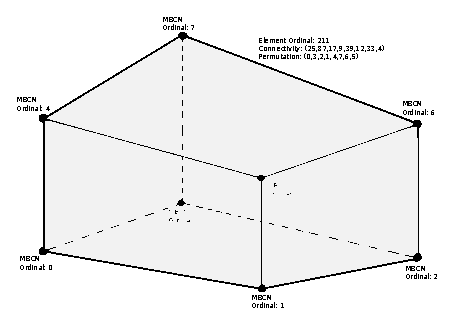
\includegraphics[width=5in]{hex_element.eps}
  \caption{\sl Basic element description for a mesh. Each element is
    required to have a unique global ordinal, and a specified
    connectivity and permuation list. The MBCN canonical ordinals used
    by DTK are specified at the nodes.}
  \label{fig:mesh_element}
\end{figure}

\subsection{Mesh Blocks}\label{subsec:blocks}
At the highest level of abstraction, the mesh is composed of mesh
blocks. These blocks contain elements of the same topology and
order. All elements in a block must have the same topology and
order. A mesh may contain as many blocks as desired. Multiple blocks
with the same mesh topology may exist. Nodes may be repeated in
different mesh blocks provided that they maintain the same unique
global ordinal and coordinates. Elements my be repeated in different
mesh blocks provided that they maintin the same unique global ordinal
and connectivity list. Multiple mesh blocks may exist in the same
spatial region as they are merely a means of subdividing the mesh into
groups of elements based on their topology. This behavior will be the
common when hybrid meshes are involved (e.g. a mesh that contains
hexahedrons and pyramids).

As an example, consider the 2 dimensional hybrid mesh presented in
figure~\ref{fig:hybrid_mesh}. This mesh contains both quadrilateral
(blue) and triangle (red) elements that share connecting nodes. In
this case, all quadrilaterals should be specified in a single mesh
block and all triangles specified in another mesh block. The nodes
shared by these two mesh blocks may be repeated in either block.

\begin{figure}[htpb!]
  \centering
  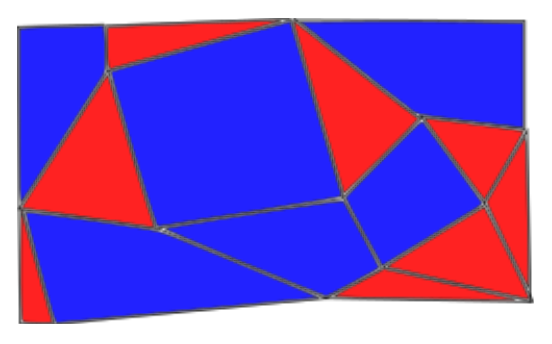
\includegraphics[width=5in]{hybrid_mesh.eps}
  \caption{\sl Hybrid mesh example. Quadrilaterals (blue) must be
    specified in a different mesh block than the triangles (red). Both
    blocks can share the mesh nodes.}
  \label{fig:hybrid_mesh}
\end{figure}

\subsection{Parallel Decomposition}\label{subsec:decomp}
Mesh blocks and the elements and nodes they contain may be partitioned
in any fashion provided that all nodes, elements, and blocks of a mesh
description exist in a communication space operated by the same
parallel communicator. Different blocks in a single mesh description
may not have different communicators. Each mesh description may have
its own communicator. Global knowledge of the parallel decomposition
of a given mesh description is not required. Only local data access
along with the proper communicator is required.

\clearpage

%%---------------------------------------------------------------------------%%
\section{Rendezvous}\label{sec:rendezvous}
Relating two non-conformal meshes will ultimately require some type of
evaluation algorithm to apply the data from one mesh to another. To
achieve this, the target objects to which this data will be applied
must be located within the the source mesh. In a serial formulation,
efficient search structures that offer logarithmic asymptotic time
complexity are available to perform this operation. However, in a
parallel formulation, if these two meshes are arbitrarily decomposed,
then a certain degree of communication will be required as well. A
mesh that is associated with the data that will be transferred will be
referred to as the source mesh while the mesh, or more generally, the
geometry that will be receiving the data will be referred to as the
target geometry.

\subsection{The Rendezvous Algorithm}\label{subsec:rendezvous_alg}
The rendezvous decomposition concept uses a parallel formulation for
the data transfer while maintaining a serial formulation for the
geometric search operations.

\clearpage

%%---------------------------------------------------------------------------%%
\section{Fields}\label{sec:field}

\subsection{Fields of Multiple Dimensions}\label{subsec:field_dim}

\subsection{Field Evaluations}\label{subsec:eval}

\clearpage

%%---------------------------------------------------------------------------%%
\section{Mesh/Field Mapping}\label{sec:map}

\clearpage

%%---------------------------------------------------------------------------%%
\section{Transfer Operations}\label{sec:transfer}

\clearpage

%%---------------------------------------------------------------------------%%
\section{Conclusion}\label{sec:conc}

%%---------------------------------------------------------------------------%%
\pagebreak
\bibliographystyle{ieeetr}
\bibliography{references}
\end{document}


